\subsection{Background}
The Corporate Partnership Programme (CPP) is a website designed to `promote the relationship between the Department of Computing and organisations who wish to recruit our students whilst investing in academic sponsorship'\cite{doc-cpp}.

In order for students to use the system they must log on, register some check box interests, and then upload their CV.
Once they have done this the student's CPP journey is complete.
Corporate Partners then log on and can browse this list of students in order to contact them regarding internships, placements, and graduate opportunities. To contact students regarding events and placements they must send an email to the CPP administrators who can then forward it on if it is deemed fit for purpose. To contact students directly they typically extract their email address from their CV.

\begin{figure}[H]\centering
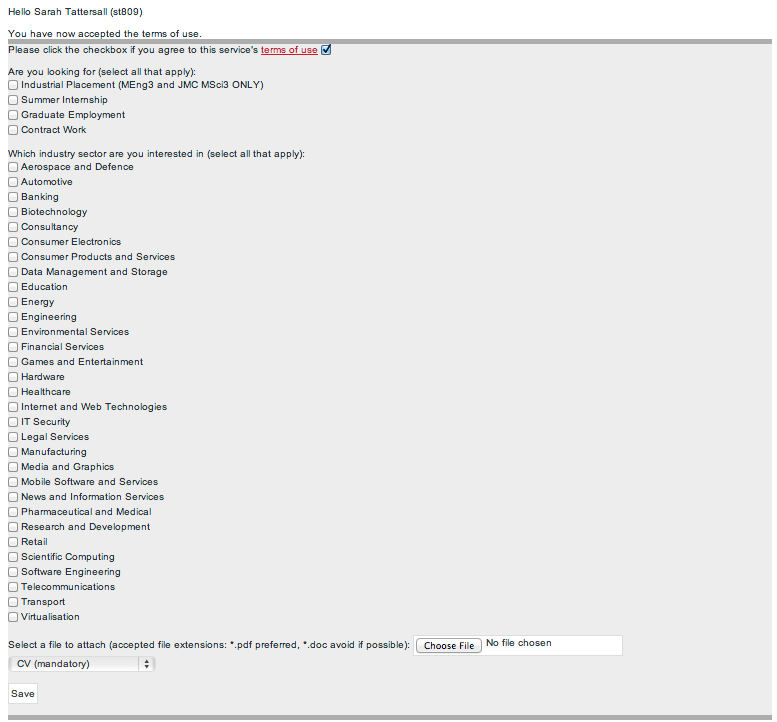
\includegraphics[scale=0.5]{images/introduction/old_cpp}
\caption{Entirety of the old site as viewable to the student}
\end{figure}
